\documentclass[tikz,border=10pt]{standalone}
% Figure: rectangle ABCQ with point P on AB and segment PQ
\begin{document}
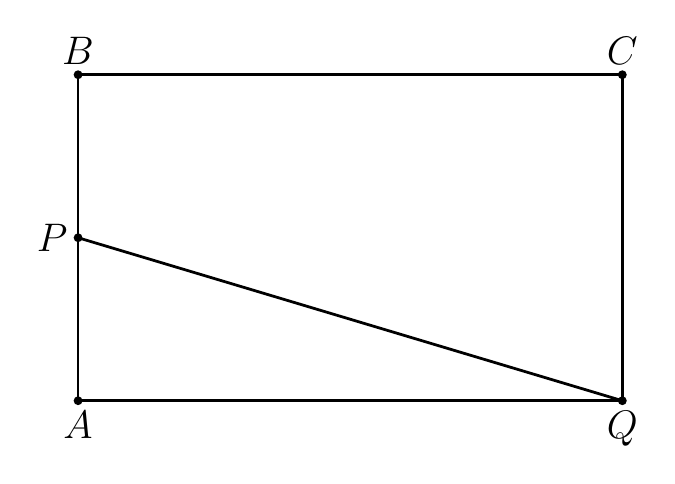
\begin{tikzpicture}[line join=round, line width=1.0pt]
  % Vertices (scale s = 0.017544 cm per px, y flipped, centred on bbox)
  \coordinate (A) at (-3.456,-2.070);
  \coordinate (B) at (-3.456, 2.070);
  \coordinate (C) at ( 3.456, 2.070);
  \coordinate (Q) at ( 3.456,-2.070);
  \coordinate (P) at (-3.456, 0.000);

  % Solid segments
  \draw (A) -- (B);
  \draw (B) -- (C);
  \draw (C) -- (Q);
  \draw (Q) -- (A);
  \draw (P) -- (Q);

  % Filled dots at the five vertices
  \fill (A) circle (1.6pt);
  \fill (B) circle (1.6pt);
  \fill (C) circle (1.6pt);
  \fill (Q) circle (1.6pt);
  \fill (P) circle (1.6pt);

  % Labels (outside the vertices)
  \node[above, font=\fontsize{14.5}{17.4}\selectfont] at (B) {$B$};
  \node[above, font=\fontsize{14.5}{17.4}\selectfont] at (C) {$C$};
  \node[below, font=\fontsize{14.5}{17.4}\selectfont] at (A) {$A$};
  \node[below, font=\fontsize{14.5}{17.4}\selectfont] at (Q) {$Q$};
  \node[left, font=\fontsize{14.5}{17.4}\selectfont] at (P) {$P$};
\end{tikzpicture}
\end{document}